\section{Izospektralni Hamiltoniani}

Izospektralni Hamiltoniani v nerelativisti\v cni kvantni mehaniki so taki, ki imajo strogo enake energijske
spektre vezanih stanj in enake transmisijske/refleksijske koeficiente sipalnih stanj. Edino, kar se
med njimi razlikuje, so valovne funkcije in posledi\v cno nekateri momenti ($\langle x \rangle$, $\langle
x^2 \rangle$ \ldots).

Ideja je ta: superpotencial $W(x)$, ki povezuje $V^{(1)}$ in $V^{(2)}$ ni enoli\v cen, zato lahko poi\v scemo
dru\v zino superpotencialov $\tilde{W}$, ki povezujejo $\tilde{V}^{(1)}$ in $V^{(2)}$. Tako dobimo dru\v zino
$\{\tilde{V}^{(1)}(x;\lambda_1)\}$, ki imajo vsi istega supersimetri\v cnega partnerja $V^{(2)}$. Da se bomo ognili
nanavadnim koeficientom bomo delali v enotah $\hbar = 2m = 1$, zaradi \v cesar se bomo iznebili raznoraznih
koeficientov $(\sqrt{2})^{\pm 1}$ (pozor, cele potence \v stevila $2$ ostanejo).

Hamiltoniani, oblike

\begin{equation}
	H = \frac{\d^2}{\d x^2} + \tilde{V}^{(1)} (x;\lambda_1),
\end{equation}

\ni so vsi izospektralni glede na parameter $\lambda_1$.

Recimo, da $W(x)$ ni enoli\v cen. Potem poleg $W(x)$ obstaja \v se $\tilde{W}(x)$, ki prav tako ustreza
en.~\eqref{v2pot}. Najpreprostej\v sa ideja bi bila potem

\begin{equation}
	W(x) \to \tilde{W}(x) = W(x) + \phi(x),
\end{equation}

\ni kjer zahtevamo, da $\tilde{W}(x)$ prav tako uboga en.~\eqref{riccati} za $V^{(2)}(x)$, ki se v teh enotah
glasi

\begin{equation}
	V^{(2)} (x) = W^2(x) + \px W(x) = \tilde{W}^2(x) + \px\tilde{W}(x),
\end{equation}

\ni od koder sledi

\begin{align}
	W^2 + \odv W &= W^2 + \odv W + 2W\phi + \odv \phi + \phi^2, \notag \\
	2W(x)\phi(x) + \phi^2(x) &= -\odv \phi (x), \notag \\
	\frac{2W(x)}{\phi(x)} + 1 &= -\frac{1}{\phi^2(x)}\odv\phi(x),\qquad y(x) = 1/\phi(x), \notag \\
	2W(x)y(x) + 1 &= -\odv y(x).
\end{align}

\ni Ko to ena\v cbo re\v simo, dobimo

\begin{equation}
	\phi(x) = \odv \ln \bigg[\int_{-\infty}^x \psi_0^2(u)\d u + \lambda_1\bigg] =
		\odv \ln \big[\mathcal{I}_1(x) + \lambda_1\big],
\end{equation}

\ni kjer je $\psi_0(x)$ spet normirana funkcija izvornega potenciala $V^{(1)} (x)$.

Dru\v zina potencialov $\tilde{V}^{(1)} (x; \lambda_1)$, ki ima partnerski potencial $V^{(2)}(x)$ je torej

\begin{equation}
	\tilde{V}^{(1)} (x;\lambda_1) = V^{(1)}(x) - 2\frac{\d^2}{\d x^2}\ln\big[\mathcal{I}_1(x) + \lambda_1\big].
\end{equation}

\ni Parameter $\lambda_1$ se je notri pri\v stulil kot integralska konstanta in ne more biti \v cisto poljuben, ampak
$\lambda_1 \notin [0,1]$, tj $\lambda_1 \in \mathbb{R}\text{\textbackslash}[-1,0]$ -- v tistem re\v zimu osnovno stanje
$\psi_0 (x; \lambda_1)$, potenciala $\tilde{V}^{(1)}(x; \lambda_1)$, ni mo\v c normirati. Izvorni potencial $V^{(1)}(x)$
dobimo kot limito $\lambda_1 \to \pm \infty$. Sliki~\ref{sl2} in~\ref{sl3} ka\v zeta primer za harmonski oscilator.

\begin{figure}[H]
	\centering
	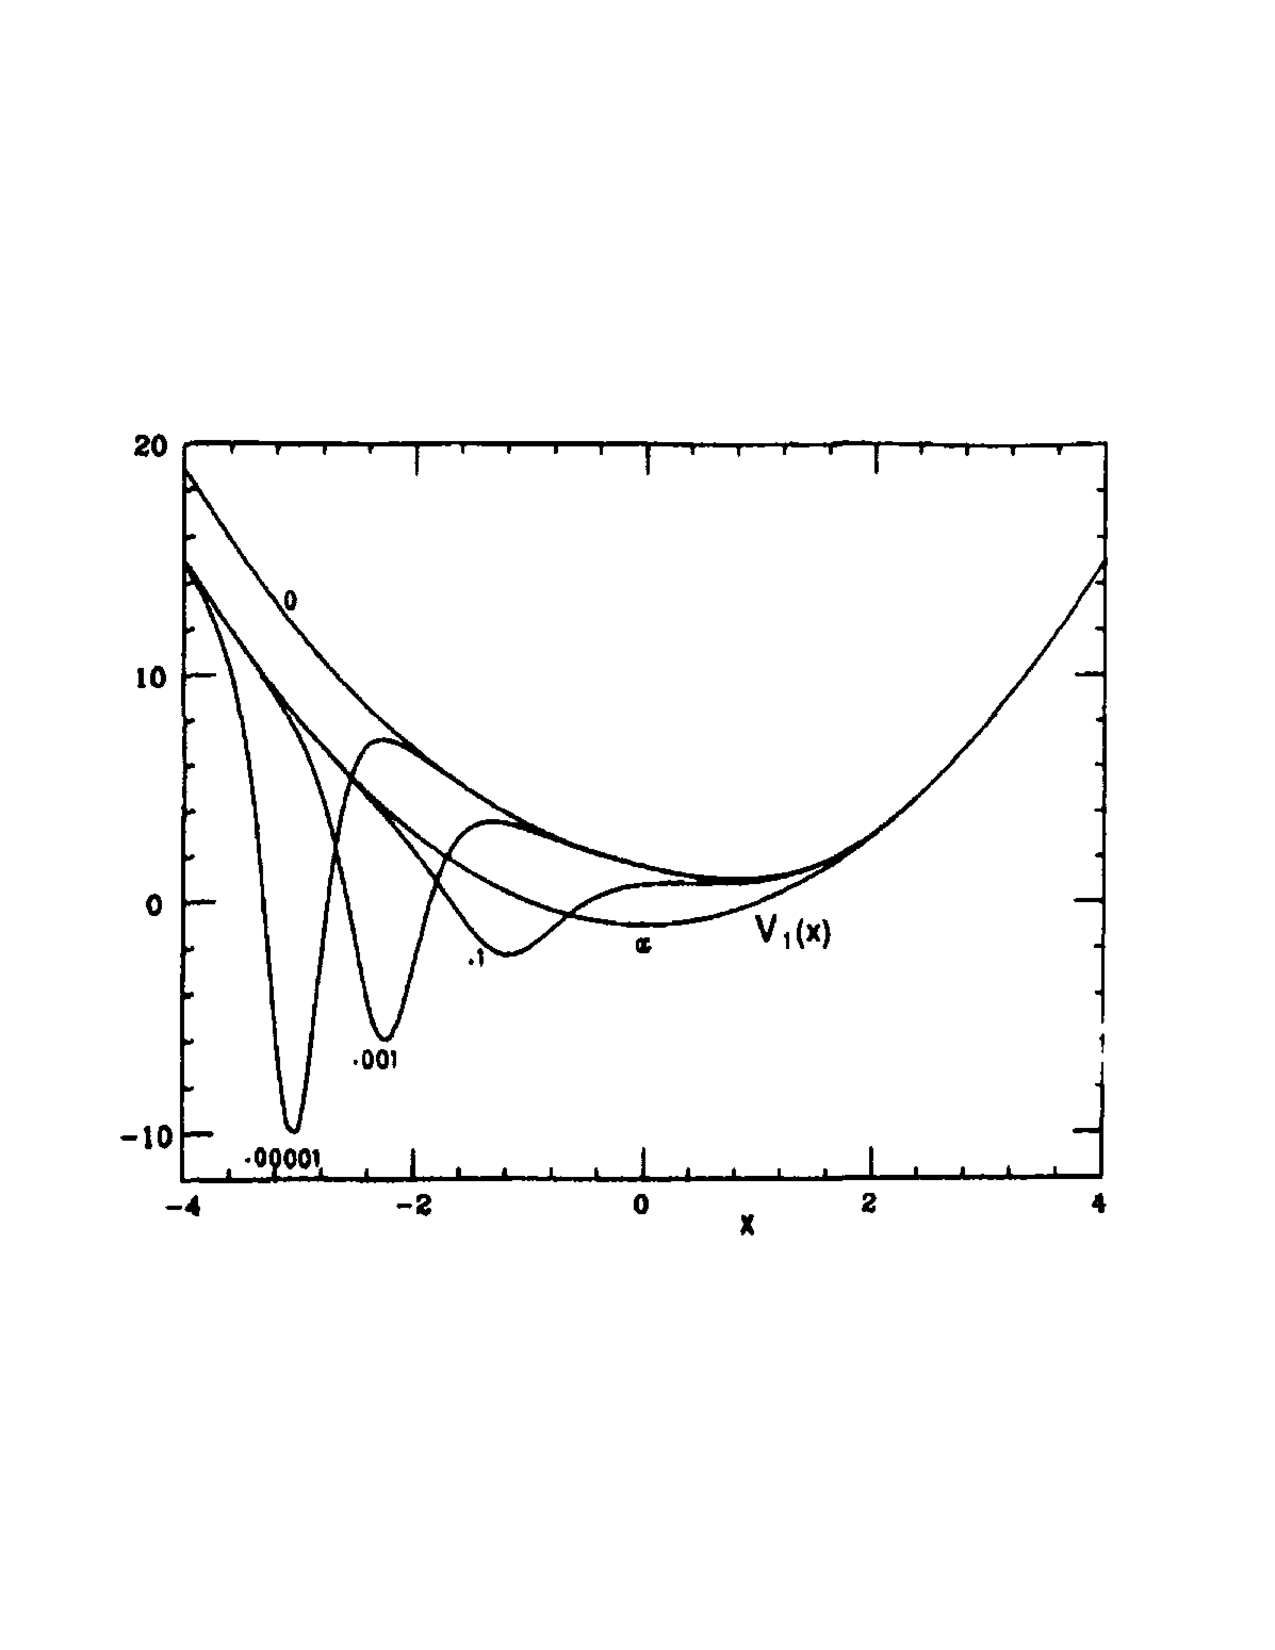
\includegraphics[height=8cm, keepaspectratio=1, trim=0cm 7cm 0cm 7cm]{pics/slika2}
	\caption{Potenciali $\tilde{V}^{(1)}$ za razli\v cne vrednosti $\lambda_1$. Izvorni $V^{(1)}$ je bil Harmonski
		oscilator, ki je tudi prikazan na grafu. Hamiltoniani s temi potenciali so popolnoma izospektralni.}
	\label{sl2}
\end{figure}

\begin{figure}[H]
	\centering
	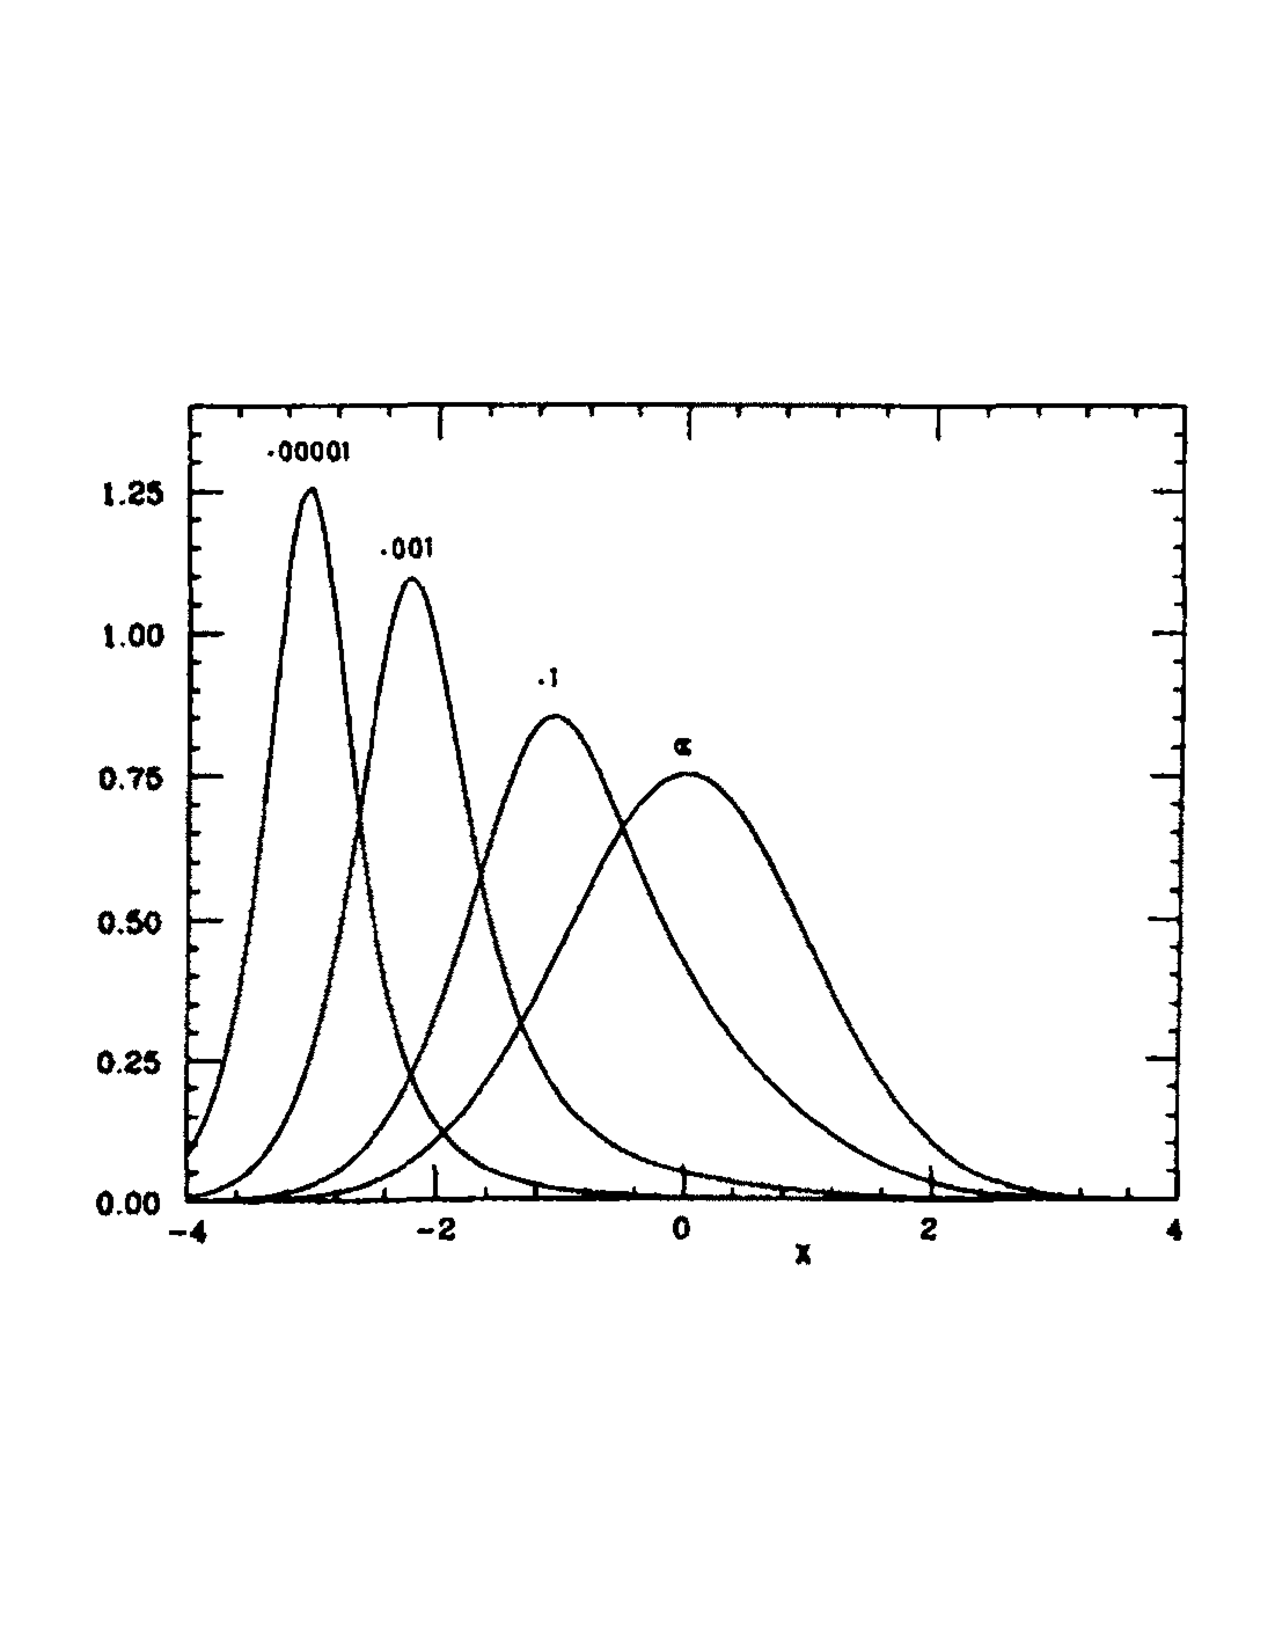
\includegraphics[height=8cm, keepaspectratio=1, trim=0cm 7cm 0cm 7cm]{pics/slika4}
	\caption{Graf prikazuje osnovne valovne funkcije k grafu iz slike~\ref{sl2}.}
	\label{sl3}
\end{figure}

Sedaj smo dobili dru\v zine potencialov, ki vrnejo vsa stanja ista, razen osnovnega, ki je odvisen od parametra $\lambda_1$.
Vendar gremo lahko korak dlje in isto naredimo za $V^{(2)}$, ki ga spremenimo v $\tilde{V}^{(2)}(x; \lambda_2)$, kar se potem
pomeni $V^{(1)} \to \tilde{V}^{(1)} (x; \lambda_1, \lambda_2)$. To lahko posplo\v simo na vsa vezana stanja in dobimo $\tilde{V}
^{(1)}(x; \underline{\lambda})$.

Taka dru\v zina potencialov, $\tilde{V}^{(1)}(x;\underline{\lambda})$, je popolnoma izospektralna, momente pa lahko nastavljamo
poljubno prek $\underline{\lambda}$.

